\chapter{Introduction}
\label{sec:intro}
\chaptermark{Introduction}

%Introduction.

\section{Segmentation and figure-ground organization}
The task of partitioning an image into regions bounded by contours (segmentation) and the task of assigning border ownership of these contours to either the foreground or the background (figure-ground organization) are important first steps in achieving image understanding. Gestalt psychologists were the first to recognize the importance of the whole in influencing perception of the parts, and with this observation, laid out several principles for figure-ground
organization\citep{Koffka35, Wertheimer23}. For example, the rule of good continuation states that well-aligned contour elements should be grouped together. This is closely related to the concept of a ''local association field,'' where collinear contour elements excite each other and noncollinear elements inhibit each other~\citep{Ullman92, Field_etal93}. Results from neuroanatomy lend support to these ideas, as the lateral connections within V1 predominantly link similar-orientation cortical columns. \textit{However, our
  understanding of the neural mechanisms of these processes remains
  surprisingly limited.}
 
The brain must keep track of which regions and contours belong to which objects. This is known as the binding problem, as it is not clear how the features of an object are bound together~\citep{Treisman96b}. One solution involves differential neural activity, where the neurons responding to the features of an
object show increased firing compared with neurons responding to the
background. This response enhancement is known as figure-ground modulation (FGM), and was first observed in primary visual cortex (V1) for texture-defined figures~\citep{Lamme95}. Similar results have been found using other tasks and techniques, including more recent voltage-sensitive dye imaging of populations of neurons during a contour grouping task~\citep{Gilad_etal13}. However, this solution only works if there is a single object in the foreground, as multiple objects each labeled with higher neural activity could be interpreted as parts of a single object. Furthermore, each neuron's firing rate is inherently ambiguous, as higher activity could be due to labeling with FGM or because the neuron's preferred feature falls within its receptive field. As a result, the binding problem cannot be solved 
with models that only represent object information in terms of enhanced neural activity in early visual areas \citep{Niebur00a}. {\em I believe that this strongly points to neural circuits that employ populations of neurons which explicitly represent (\ie in their firing rate) the organization of the visual scene in terms of perceptual objects.}

\section{The role of cortical feedback}
The degree of collinear facilitation observed in V1 is strongly context-dependent, and can change with the behavioral task~\citep{Li_etal04, Li_etal06} as well as perceptual learning~\citep{Li_etal08a, Yan_etal14}. As a result, feedback connections from higher areas may play an important role in shaping the responses of neurons in early visual areas. In fact, simultaneous neural recordings from areas V1 and V4 during two different figure-ground segregation tasks show that V4 is intimately involved in the FGM process~\citep{Poort_etal12, Chen_etal14}. In these studies, the FGM signal appears first in V4 and is then fed back to V1, with a delay representing recurrent processing. Additional studies of curve-tracing~\citep{Roelfsema_etal98} and border ownership~\citep{Zhou_etal00, Qiu_etal07, Zhang_vonderHeydt10} further
demonstrate that feedback mechanisms are necessary for explaining FGM
in the presence of multiple objects. \textit{However, essential  questions still remain about the nature of the interactions between  and within different cortical areas.} How is early-level feature information about an object combined with global context information about the object in a synergistic way in order to generate FGM?

\section{The role of attention}
Behavioral studies have shown that attention can be directed to objects \citep{Egly_etal94} and electrophysiological results demonstrate that attention can act as a top-down signal which influences FGM~\citep{Qiu_etal07,  Poort_etal12}. In an ambiguous figure-ground display, attending to one region increases the probability that this region is perceived as figure~\citep{Driver_Baylis96, Vecera_etal04}. Spatial attention, which has been extensively studied, acts like a ''spotlight'' that enhances neural responses within the focus of attention and suppresses responses outside~\citep{Motter93a}. Attention can also operate in a feature-based or object-based manner. Feature-based attention acts broadly across the visual scene and increases the responses of all components that share similar feature attributes (e.g. color, orientation, or direction of movement) with the attended component~\citep{Treue_Trujillo99}. Object-based attention highlights all the parts of an object, also encompassing all the features that belong to the object~\citep{Roelfsema_etal98, Schoenfeld_etal14}.
Attention has been found to modulate border ownership in an object-based manner~\citep{Qiu_etal07}. Border ownership is a property of many neurons in V2 which encodes the side to which an object border
belongs relative to their receptive field \citep{Zhou_etal00}. To explain these results,~\citet{Craft_etal07} proposed a model in which populations of grouping neurons explicitly represent (in their firing rates) the perceptual organization of the visual scene. Grouping neurons are reciprocally connected to border ownership selective (BOS) neurons through feedforward and feedback connections. Attention broadly
targets grouping neurons, which can then modulate the activity of BOS
neurons through feedback~\citep{Mihalas_etal11b}. A feedforward version of this model has been applied to natural images, where it outperforms other models in predicting the location of eye
fixations~\citep{Russell_etal14}.

The proposed project explains perceptual organization by a combination
of top-down and lateral interactions in visual cortex. The interest in the mechanisms of perceptual organization related to visual (not cognitive~) top-down information over the last years was sparked by
the co-sponsor's discovery of border ownership selectivity in extrastriate cortex~\citep{Zhou_etal00}. A series of subsequent physiological findings \citep{vonderHeydt_etal00a,vonderHeydt_etal03b,Qiu_vonderHeydt05,vonderHeydt_etal05,vonderHeydt_Pierson06,Qiu_vonderHeydt07,Qiu_etal07,OHerron_vonderHeydt09,
  Zhang_vonderHeydt10,Sugihara_etal11,OHerron_vonderHeydt13} and
computational results \citep{Dong_etal08a,Craft_etal07,Mihalas_etal11b,Ardila_etal12,Russell_etal14} elaborated many details of these mechanisms.  The sponsor has a
long-standing interest in the role of intra-areal lateral (``horizontal'') connections in early visual cortex in the representation of contours. The resulting computational model developed by \citet{Stemmler_etal95b} has since been corroborated by a large number of independent studies
\citep[e.g.][]{Simonotto_etal97,Polat_etal98,Chatterjee_etal11,Xie_etal14}. However, in agreement with others at the time, the underlying concept of horizontal connections in that model was that they are essentially static, or varying over time scales given by ontogenetic development or neuronal plasticity. Such structures could thus implement overall statistics of natural scenes~\citep[like circular structures, e.g.][]{Sigman_etal01} but they could not flexibly represent the myriad of instantaneously present and constantly changing visual shapes observed during perception of dynamic scenes. This view has been considerably enlarged over the last decade or so, with the~\citet{Chen_etal14} article, on which Brian bases a large part of his model, being the latest in a series of psychophysical and physiological studies. What is emerging is a view in which the lateral connections are in place but can be actively and rapidly modulated by top-down connectivity from higher areas. It may thus be that two ``classical'' approaches to explain perceptual organization, one using the horizontal connections as a substrate~\citep[e.g.][]{Zhaoping05, Piech_etal13}, the other using white-matter projections from higher areas \citep[e.g.][]{Craft_etal07,Mihalas_etal11b}, can be converged into an integrated model.

\textbf{Contributions of this project.}  \textit{This project has the
  potential to deepen and extend our understanding of the neural
  mechanisms of FGM.} 
Most existing models~\citep{Grossberg94, Grossberg97, Zhaoping05, Piech_etal13} group object features by a diffusion-like process that propagates neural activity along lateral connections within early visual areas. Another class of models relies on the fast temporal coding structures of spike trains \citep{Singer99b}, but experimental evidence is controversial \citep{Thiele_Stoner03,Roelfsema_etal04,Dong_etal08a}.In my proposed model, FGM involves grouping mechanisms that make use of feedforward, feedback, and lateral connections between and within multiple cortical areas. Previous models on the neural coding of border ownership have identified a plausible network architecture for perceptual organization and object-based attention. I will extend these models to explain how feedback grouping mechanisms could be used to perform segmentation of both artificial and natural images. My model will also offer several falsifiable predictions which can be used to test it
and compare it with competing computational models. \textit{This study also has implications for patients with object-based neglect.} Patients who exhibit this type of neglect are unable to process certain parts of an object due to lesions in higher areas of the
brain~\citep{Marshall_Halligan93}. Clarifying how top-down attention
interacts with the neural circuits responsible for grouping together
the features of an object could guide therapies for individuals with
object-based neglect.

Grouping mechanisms are important not only for piecing together object
contours, but also for providing a structure for selectively attending
to groups of objects~\citep{Treisman_Gelade80}. Supported by extensive
psychophysical data,~\citet*{Nakayama_etal95} proposed that surface
representations play a key role in intermediate-level vision. For
example, by selectively attending to a surface in 3D space, subjects
can perform efficient search for a conjunction target~\citep{Nakayama_Silverman86}. In a separate cueing experiment,
attention was shown to spread automatically across surfaces~\citep{He_Nakayama95}. These abilities indicate powerful
mechanisms for grouping objects into surfaces in 3D space, and suggest
that structuring the world in terms of surfaces might be an ecologically important function (\eg for locomotion along the ground
plane, reaching for objects along a table top \etc). I hope to show that basis functions provide a suitable theoretical framework for studying how top-down signals, including those used by grouping and attentional mechanisms, may interact with feedforward and lateral connections to dynamically modify the responses of feature-selective
neurons in a surface-based manner. \textit{I believe that my models will provide insight into the neural circuits that represent surfaces, filling a critical gap in our understanding of intermediate-level vision.}

\section{Overview of the grouping model}
\begin{figure}[t]
\centering
\includegraphics[width=\textwidth]{Intro/figs/groupingcircuit}
\makeatletter
\let\@currsize\normalsize
\caption{Grouping model}
\label{fig:GroupingModel}
\end{figure}

Several models have been proposed~\citep{Zhaoping05, Sakai_Nishimura06,Craft_etal07, Layton_etal12} to describe how a neuron's border ownership selectivity can be modulated by visual input far away from its classical receptive field (RF). In the grouping model
\citep{Craft_etal07}, BOS neurons participate in neural circuits that define perceptual objects early-on in processing (Figure~\ref{fig:GroupingModel}). An object border activates a pair of orientation-selective BOS neurons whose RFs are shown as ellipses. The arrows on the RFs point towards the preferred direction of the neuron, indicating where the object is relative to the neuron's RF. BOS neurons activated by the solid-line square (red ellipses) excite the appropriate grouping neuron (red G in circle) through feedforward connections (red solid lines). The grouping neuron in turn enhances the activity of the same BOS neurons through feedback connections (red dotted lines). This type of facilitatory feedback may be mediated by NMDAR channels, which allow gating of sensory input by top-down signals~\citep{Palmer_etal14}. Neurons consistent with other objects (e.g. the dashed-line square) project to other grouping neurons (blue G in circle in this case). Presence of the solid-line square increases the firing rate of the red grouping neuron over that of the blue (and other) grouping neurons since the latter receive less feedforward input. As a consequence, the red grouping neuron provides more feedback to the red BOS neurons than the blue and gray BOS neurons would receive from their respective grouping neurons. Likewise, presence of the dashed-line square increases the firing rates of all blue neurons over those of gray and red neurons. Thus, an object border is represented by two BOS neurons whose relative activity codes for the side of ownership. The relative difference in firing rate is also known as the BOS signal~\citep{Zhou_etal00}.

The BOS signal appears \textasciitilde 25 ms after the visual response
to an oriented edge, and the delay is essentially independent of object size \citep{Zhou_etal00}. This constant delay is consistent with a model in which grouping neurons of different sizes integrate local edge signals, and by feedback enhance the same edge
 signals~\citep{Craft_etal07}. Attention enhances a BOS neuron's
 response when an object is on the neuron's preferred side, but has a
 suppressive effect if the object is on the non-preferred
 side~\citep{Qiu_etal07}. This asymmetry is consistent with a model in
 which top-down attention targets grouping neurons, which then modulate
 the activity of BOS neurons through feedback~\citep{Mihalas_etal11b}. Additional support for the grouping model comes from observations of short-term memory of BOS signals~\citep{OHerron_vonderHeydt09} and remapping of BOS signals across saccades and object movements~\citep{OHerron_vonderHeydt13}. These findings are difficult
 to explain with models that only represent object information in terms
 of neural activity in early visual areas. I believe that this strongly
 points to neural circuits that employ populations of neurons which
 explicitly represent (\ie in their firing rate) the organization of
 the visual scene.

%%% Local Variables:
%%% mode: latex
%%% TeX-master: "../root"
%%% End:
